\documentclass[a4paper, 10pt]{article}
\usepackage{helvet}
\renewcommand{\familydefault}{\sfdefault}
\usepackage{pgf}
\usepackage{eurosym}
\usepackage{graphicx}
\usepackage{wasysym}
\usepackage{hyperref}
\usepackage{listings}
\usepackage{pxfonts}
\usepackage{verbatim}
\usepackage{color}
\usepackage{xcolor}
\usepackage{wrapfig}
\usepackage{enumitem}
\usepackage{booktabs}
\usepackage{gensymb}
\usepackage{tabularx}
\usepackage{currfile}

\hypersetup{
    bookmarks=true,         % show bookmarks bar?
    unicode=true,          % non-Latin characters in Acrobat’s bookmarks
    pdftoolbar=true,        % show Acrobat’s toolbar?
    pdfmenubar=true,        % show Acrobat’s menu?
    pdffitwindow=true,     % window fit to page when opened
    pdftitle={Assessments},    % title
    pdfauthor={Paul Vesey},     % author
    pdfsubject={Building Information Modelling },   % subject of the document
    pdfcreator={},   % creator of the document
    pdfproducer={xelatex}, % producer of the document
    pdfkeywords={'Graphics' }, % list of keywords
    pdfnewwindow=true,      % links in new PDF window
    colorlinks=true,       % false: boxed links; true: colored links
    linkcolor=violet,          % color of internal links (change box color with linkbordercolor)
    citecolor=magenta,        % color of links to bibliography
    filecolor=red,      % color of file links
    urlcolor=blue           % color of external links
}

\setlength\parindent{0pt}
\begin{document}

\lstset{language=HTML,
				basicstyle=\small,
				breaklines=true,
        numbers=left,
        numberstyle=\tiny,
        showstringspaces=false,
        aboveskip=-20pt,
        frame=leftline
        }
				
\begin{figure}
	\centering
	
\includegraphics[width=0.5\linewidth]{./Assignments/img/LITlogo}
\end{figure}


\begin{tabularx}{\textwidth}{ |l|X| }
	\hline
	\textbf{Subject:} & Revit MEP\\
	\textbf{Course:} & Building Information Modelling with Revit MEP\\
	\textbf{Session:} & Autumn 2021\\
	\textbf{Lecturer:} & Paul Vesey \footnotesize{BEng, MIE, HDip}\\
	\textbf{Filename:} & \currfilebase\\
	\hline
\end{tabularx}



\vspace{0.25cm}	
	
\begin{flushleft}
\Large\textbf{Assignment 1 (33\%) - Detached 2 Storey Residence with Dormer Window}\\
\end{flushleft}

\begin{tabular}{|l|l|}
	\hline 
	Issue Date & As per Moodle \\ 
	\hline 
	Submission Date & As per Moodle \\ 
	\hline 
\end{tabular} 
\\

\large\textbf{Assignment Outline}\\

You are required to model a two storey house incorporating a dormer window and to digitally submit you project file (.rvt) showing your model on one A4 sheet and three A1 sheets.

\large\textbf{Your Submission should contain the following information}\\


\textbf{Sheet 1:} Sheet Size - A4, Sheet No - A101, Sheet Name - Cover Sheet
\begin{itemize}
	\item Three Dimensional (Aerial View) of the model (scaled to suit the sheet size) Shaded
	\item A list of the drawings in the design pack
\end{itemize}


\textbf{Sheet 2:} Sheet Size - A1, Sheet No - A102, Sheet Name - Floor Plans
\begin{itemize}
	\item Ground and First Floor Plans @ 1:50 with dimensions, Room Titles ans some fixed furniture
	\item Two internal camera views, (scaled to suit the sheet size) rendered using the Autodesk 360 cloud rendering service.  \textit{One of the fireplace and one of the kitchen units} 
\end{itemize}


\textbf{Sheet 3:} Sheet Size - A1, Sheet No - A103, Sheet Name - Elevations
\begin{itemize}
	\item South Elevation @ 1:50
	\item North, East and West Elevations @ 1:100
\end{itemize}

\textbf{Sheet 4:} Sheet Size - A1, Sheet No - A102, Sheet Name - Sections and Details
\begin{itemize}
	\item Three sections are required
	\item Section thro' Kitchen / Sitting Room facing East (towards fireplace) @ 1:100
	\item Section thro' Kitchen / Sitting Room facing West (towards kitchen units) @ 1:100
	\item Section thro' the Hallway / Landing showing the Stairs and the Dormer @ 1:100
	\item One full height detail (Call-outs) @ 1:20, including Repeating Details showing the following:
	\begin{itemize}
		\item Foundation / External Wall / Floor Interfaces
		\item Facia / Soffit and Roof Details
		\item All necessary notes
	\end{itemize} 
\end{itemize}

Additional Sheets may be submitted if so desired.

\large\textbf{Presentation and Submission}\\
\begin{enumerate}
	\item All drawing sheets must have the LIT Built Environment logo and be clearly marked 'Educational Exercise - Not for Construction
	\item You are required to submit you project as a single Revit (.rvt) file through Moodle
	\item Drawings should show all necessary information to communicate design intent
	\item The Revit filename should be of the form \textit{Semester  + Year + Project No. + First Initial + Surname + K-Number}. An example would be \textbf{'Spring18P01PVeseyK00123456.rvt'}.  Do not use spaces in the filename
\end{enumerate}


\textbf{How to Structure your Submission}
\\
All submission are to take the form of a single zip file.  The zip file must maintain the folder structure as generated by 3DS Max or Unity.   The images below, figure \ref{fig:3dsstructure} and figure \ref{fig:unity} give an indication of the folder structure that you should zip and submit.\\ \\

\begin{figure}[h]
	\centering
	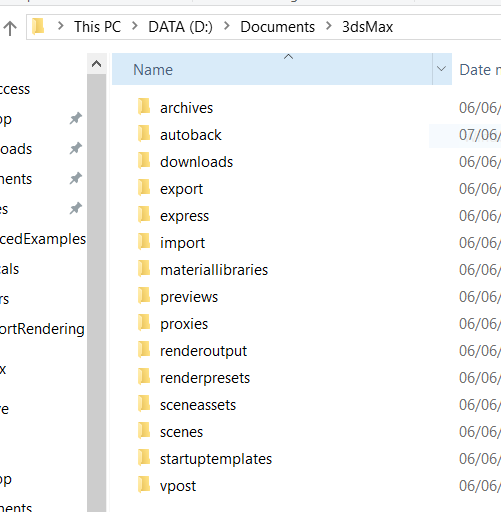
\includegraphics[width=0.5\linewidth]{img/3dsStructure.jpg}
	\caption{3D Studio Max Project Folder Structure}
	\label{fig:3dsstructure}
\end{figure}
\begin{figure}[h]
	\centering
	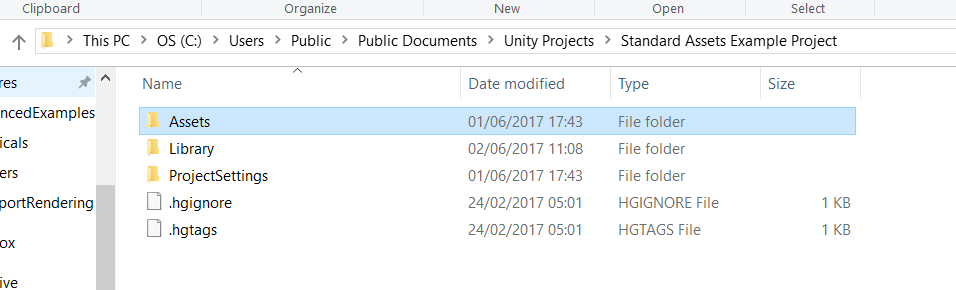
\includegraphics[width=0.9\linewidth]{img/Unity.jpg}
	\caption{Unity Game Engine File Structure}
	\label{fig:unity}
\end{figure}

All assets used during the course of the assignment are to be submitted.  All assets used and created should be placed within the appropriate folder.  To clarify, all 3ds Scene files should be placed within the 'scenes' folder; and all renders should be placed within the 'renderoutput' folder.
\\
\\
Please note that it is not appropriate to submit a single \textit{.max} file, single \textit{.jpg} file, or a single \textit{.unity} file.  

\vspace{1cm}
\textbf{Late Submission}\\
Failure to submit your assignment on or before the date and time indicated will result in a penalty of 5\% per day or part thereof.
\\
\\
Late submission penalties will not apply in cases where a valid medical certificate is provided.  In such instances an extension of time will be granted for the duration of illness stated on the medical certificate that falls after the submission date.  A copy of the medical certificate must be included with the late submission.
\\
\\
Late submission penalties may also be avoided in exceptional circumstances.  These will be dealt with on a case by case basis.  Please note that loss of pen-drives, inability to use or access the software etc. will not be considered 'exceptional circumstances'.




\end{document}